

\section{parsetree}

\textit{module Parsetree} and \textit{module parsetree}
defined abstract syntax tree produced by parsing.

\begin{figure}
  \centering
  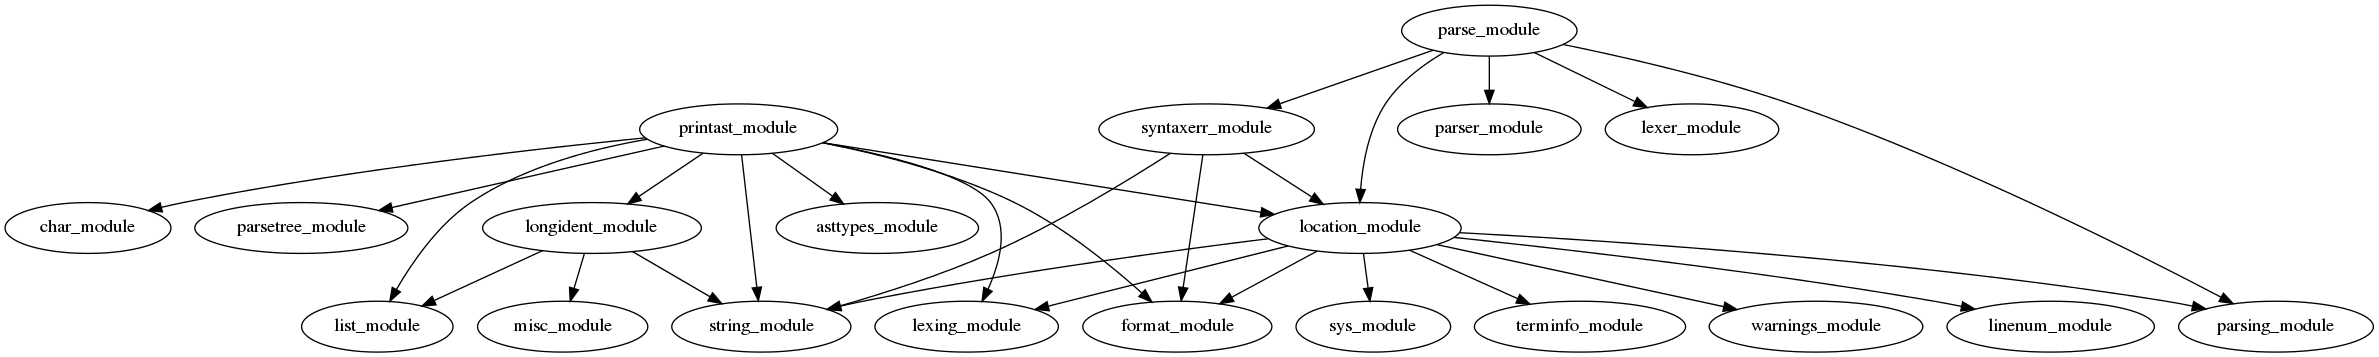
\includegraphics[scale=0.2,angle=-90]{graphics/parsing_dep.png}
  \caption{parsing depdency}
  \label{fig:parsing_dep}
\end{figure}


\begin{ocamlcode}
type constant =
    Const_int of int
  | Const_char of char
  | Const_string of string
  | Const_float of string
  | Const_int32 of int32
  | Const_int64 of int64
  | Const_nativeint of nativeint
type rec_flag = Nonrecursive | Recursive | Default
type direction_flag = Upto | Downto
type private_flag = Private | Public
type mutable_flag = Immutable | Mutable
type virtual_flag = Virtual | Concrete
type override_flag = Override | Fresh
type closed_flag = Closed | Open
type label = string
\end{ocamlcode}
\captionof{listing}{asttypes \label{asttypes}}

\newpage
\inputminted[fontsize=\scriptsize]{ocaml}{code/compiler/ast.ml}
\captionof{listing}{ocaml parsing ast}

